% Options for packages loaded elsewhere
\PassOptionsToPackage{unicode}{hyperref}
\PassOptionsToPackage{hyphens}{url}
%
\documentclass[
]{book}
\usepackage{amsmath,amssymb}
\usepackage{lmodern}
\usepackage{iftex}
\ifPDFTeX
  \usepackage[T1]{fontenc}
  \usepackage[utf8]{inputenc}
  \usepackage{textcomp} % provide euro and other symbols
\else % if luatex or xetex
  \usepackage{unicode-math}
  \defaultfontfeatures{Scale=MatchLowercase}
  \defaultfontfeatures[\rmfamily]{Ligatures=TeX,Scale=1}
\fi
% Use upquote if available, for straight quotes in verbatim environments
\IfFileExists{upquote.sty}{\usepackage{upquote}}{}
\IfFileExists{microtype.sty}{% use microtype if available
  \usepackage[]{microtype}
  \UseMicrotypeSet[protrusion]{basicmath} % disable protrusion for tt fonts
}{}
\makeatletter
\@ifundefined{KOMAClassName}{% if non-KOMA class
  \IfFileExists{parskip.sty}{%
    \usepackage{parskip}
  }{% else
    \setlength{\parindent}{0pt}
    \setlength{\parskip}{6pt plus 2pt minus 1pt}}
}{% if KOMA class
  \KOMAoptions{parskip=half}}
\makeatother
\usepackage{xcolor}
\usepackage{color}
\usepackage{fancyvrb}
\newcommand{\VerbBar}{|}
\newcommand{\VERB}{\Verb[commandchars=\\\{\}]}
\DefineVerbatimEnvironment{Highlighting}{Verbatim}{commandchars=\\\{\}}
% Add ',fontsize=\small' for more characters per line
\usepackage{framed}
\definecolor{shadecolor}{RGB}{248,248,248}
\newenvironment{Shaded}{\begin{snugshade}}{\end{snugshade}}
\newcommand{\AlertTok}[1]{\textcolor[rgb]{0.94,0.16,0.16}{#1}}
\newcommand{\AnnotationTok}[1]{\textcolor[rgb]{0.56,0.35,0.01}{\textbf{\textit{#1}}}}
\newcommand{\AttributeTok}[1]{\textcolor[rgb]{0.77,0.63,0.00}{#1}}
\newcommand{\BaseNTok}[1]{\textcolor[rgb]{0.00,0.00,0.81}{#1}}
\newcommand{\BuiltInTok}[1]{#1}
\newcommand{\CharTok}[1]{\textcolor[rgb]{0.31,0.60,0.02}{#1}}
\newcommand{\CommentTok}[1]{\textcolor[rgb]{0.56,0.35,0.01}{\textit{#1}}}
\newcommand{\CommentVarTok}[1]{\textcolor[rgb]{0.56,0.35,0.01}{\textbf{\textit{#1}}}}
\newcommand{\ConstantTok}[1]{\textcolor[rgb]{0.00,0.00,0.00}{#1}}
\newcommand{\ControlFlowTok}[1]{\textcolor[rgb]{0.13,0.29,0.53}{\textbf{#1}}}
\newcommand{\DataTypeTok}[1]{\textcolor[rgb]{0.13,0.29,0.53}{#1}}
\newcommand{\DecValTok}[1]{\textcolor[rgb]{0.00,0.00,0.81}{#1}}
\newcommand{\DocumentationTok}[1]{\textcolor[rgb]{0.56,0.35,0.01}{\textbf{\textit{#1}}}}
\newcommand{\ErrorTok}[1]{\textcolor[rgb]{0.64,0.00,0.00}{\textbf{#1}}}
\newcommand{\ExtensionTok}[1]{#1}
\newcommand{\FloatTok}[1]{\textcolor[rgb]{0.00,0.00,0.81}{#1}}
\newcommand{\FunctionTok}[1]{\textcolor[rgb]{0.00,0.00,0.00}{#1}}
\newcommand{\ImportTok}[1]{#1}
\newcommand{\InformationTok}[1]{\textcolor[rgb]{0.56,0.35,0.01}{\textbf{\textit{#1}}}}
\newcommand{\KeywordTok}[1]{\textcolor[rgb]{0.13,0.29,0.53}{\textbf{#1}}}
\newcommand{\NormalTok}[1]{#1}
\newcommand{\OperatorTok}[1]{\textcolor[rgb]{0.81,0.36,0.00}{\textbf{#1}}}
\newcommand{\OtherTok}[1]{\textcolor[rgb]{0.56,0.35,0.01}{#1}}
\newcommand{\PreprocessorTok}[1]{\textcolor[rgb]{0.56,0.35,0.01}{\textit{#1}}}
\newcommand{\RegionMarkerTok}[1]{#1}
\newcommand{\SpecialCharTok}[1]{\textcolor[rgb]{0.00,0.00,0.00}{#1}}
\newcommand{\SpecialStringTok}[1]{\textcolor[rgb]{0.31,0.60,0.02}{#1}}
\newcommand{\StringTok}[1]{\textcolor[rgb]{0.31,0.60,0.02}{#1}}
\newcommand{\VariableTok}[1]{\textcolor[rgb]{0.00,0.00,0.00}{#1}}
\newcommand{\VerbatimStringTok}[1]{\textcolor[rgb]{0.31,0.60,0.02}{#1}}
\newcommand{\WarningTok}[1]{\textcolor[rgb]{0.56,0.35,0.01}{\textbf{\textit{#1}}}}
\usepackage{longtable,booktabs,array}
\usepackage{calc} % for calculating minipage widths
% Correct order of tables after \paragraph or \subparagraph
\usepackage{etoolbox}
\makeatletter
\patchcmd\longtable{\par}{\if@noskipsec\mbox{}\fi\par}{}{}
\makeatother
% Allow footnotes in longtable head/foot
\IfFileExists{footnotehyper.sty}{\usepackage{footnotehyper}}{\usepackage{footnote}}
\makesavenoteenv{longtable}
\usepackage{graphicx}
\makeatletter
\def\maxwidth{\ifdim\Gin@nat@width>\linewidth\linewidth\else\Gin@nat@width\fi}
\def\maxheight{\ifdim\Gin@nat@height>\textheight\textheight\else\Gin@nat@height\fi}
\makeatother
% Scale images if necessary, so that they will not overflow the page
% margins by default, and it is still possible to overwrite the defaults
% using explicit options in \includegraphics[width, height, ...]{}
\setkeys{Gin}{width=\maxwidth,height=\maxheight,keepaspectratio}
% Set default figure placement to htbp
\makeatletter
\def\fps@figure{htbp}
\makeatother
\setlength{\emergencystretch}{3em} % prevent overfull lines
\providecommand{\tightlist}{%
  \setlength{\itemsep}{0pt}\setlength{\parskip}{0pt}}
\setcounter{secnumdepth}{5}
\usepackage{booktabs}
\ifLuaTeX
  \usepackage{selnolig}  % disable illegal ligatures
\fi
\usepackage[]{natbib}
\bibliographystyle{plainnat}
\IfFileExists{bookmark.sty}{\usepackage{bookmark}}{\usepackage{hyperref}}
\IfFileExists{xurl.sty}{\usepackage{xurl}}{} % add URL line breaks if available
\urlstyle{same} % disable monospaced font for URLs
\hypersetup{
  pdftitle={行動経済学の実証分析},
  pdfauthor={Tomohisa OKADA},
  hidelinks,
  pdfcreator={LaTeX via pandoc}}

\title{行動経済学の実証分析}
\author{Tomohisa OKADA}
\date{2023-05-10}

\begin{document}
\maketitle

{
\setcounter{tocdepth}{1}
\tableofcontents
}
\hypertarget{ready}{%
\chapter{Ready?}\label{ready}}

\hypertarget{rstudioux3068ux306f}{%
\section{R(Studio)とは?}\label{rstudioux3068ux306f}}

\begin{itemize}
\tightlist
\item
  Rは、オープンソースで利用可能な統計解析に特化したプログラミング言語
\item
  RStudioは、Rを使うための統合開発環境(なくてもRは使えるが、あるとめちゃ便利!)\\
\item
  今は「まったく意味不明」で全然OK!
\end{itemize}

\hypertarget{tips}{%
\section{Tips!}\label{tips}}

\begin{itemize}
\tightlist
\item
  Rに関するお役立ちサイトや書籍をまとめる
\end{itemize}

\begin{enumerate}
\def\labelenumi{\arabic{enumi}.}
\item
  \href{https://tomoecon.github.io/R_for_graduate_thesis/}{「卒業論文のためのR入門」 by 森知晴先生}\\
  Rの使い方と心理統計学の基礎が一挙に学べる!
\item
  \href{https://www.jaysong.net/RBook/datahandling1.html}{「私たちのR」 by 宋財泫先生 \& 矢内勇生先生}\\
  辞書的に使える!Tidyverseを使ったモダンなRのプログラムが学べる!
\item
  \href{http://www.f.waseda.jp/sakas/R/index.html}{「経営工学雑記帖」内のRのページ by 逆瀬川浩孝先生}\\
  網羅的でスッキリわかりやすい!辞書的に使うのにオススメ
\item
  \href{https://htsuda.net/stats/}{「Rによる統計入門」 by 津田裕之先生}\\
  Rの基礎から簡単な統計分析まで(因子分析もカバー)
\item
  \href{https://shohei-doi.github.io/quant_polisci/index.html}{「Rで計量政治学入門」 by 土井翔平先生}\\
  政治学の研究者以外にも有用!特にデータの読み込みやtidyverseの使い方が詳しい!
\end{enumerate}

\hypertarget{rstudioux306eux30a4ux30f3ux30b9ux30c8ux30fcux30eb}{%
\section{R(Studio)のインストール}\label{rstudioux306eux30a4ux30f3ux30b9ux30c8ux30fcux30eb}}

\begin{itemize}
\tightlist
\item
  次のサイトにアクセス( \url{https://posit.co/download/rstudio-desktop/} )
\item
  「1:Install R」からRをインストール
\item
  「2:Install RStudio」からRStudioをインストール
\item
  うまくインストールできない場合は、\href{https://www.jaysong.net/RBook/installation.html}{「私たちのR」}に超詳しい解説がある
\end{itemize}

\hypertarget{go}{%
\chapter{Go!!}\label{go}}

\begin{itemize}
\tightlist
\item
  とりあえずまずは使ってみよう!
\end{itemize}

\hypertarget{rstudioux3092ux958bux304f}{%
\section{RStudioを開く}\label{rstudioux3092ux958bux304f}}

\begin{itemize}
\tightlist
\item
  RStudioのアイコンから起動
\item
  次のような画面が表示される\\
  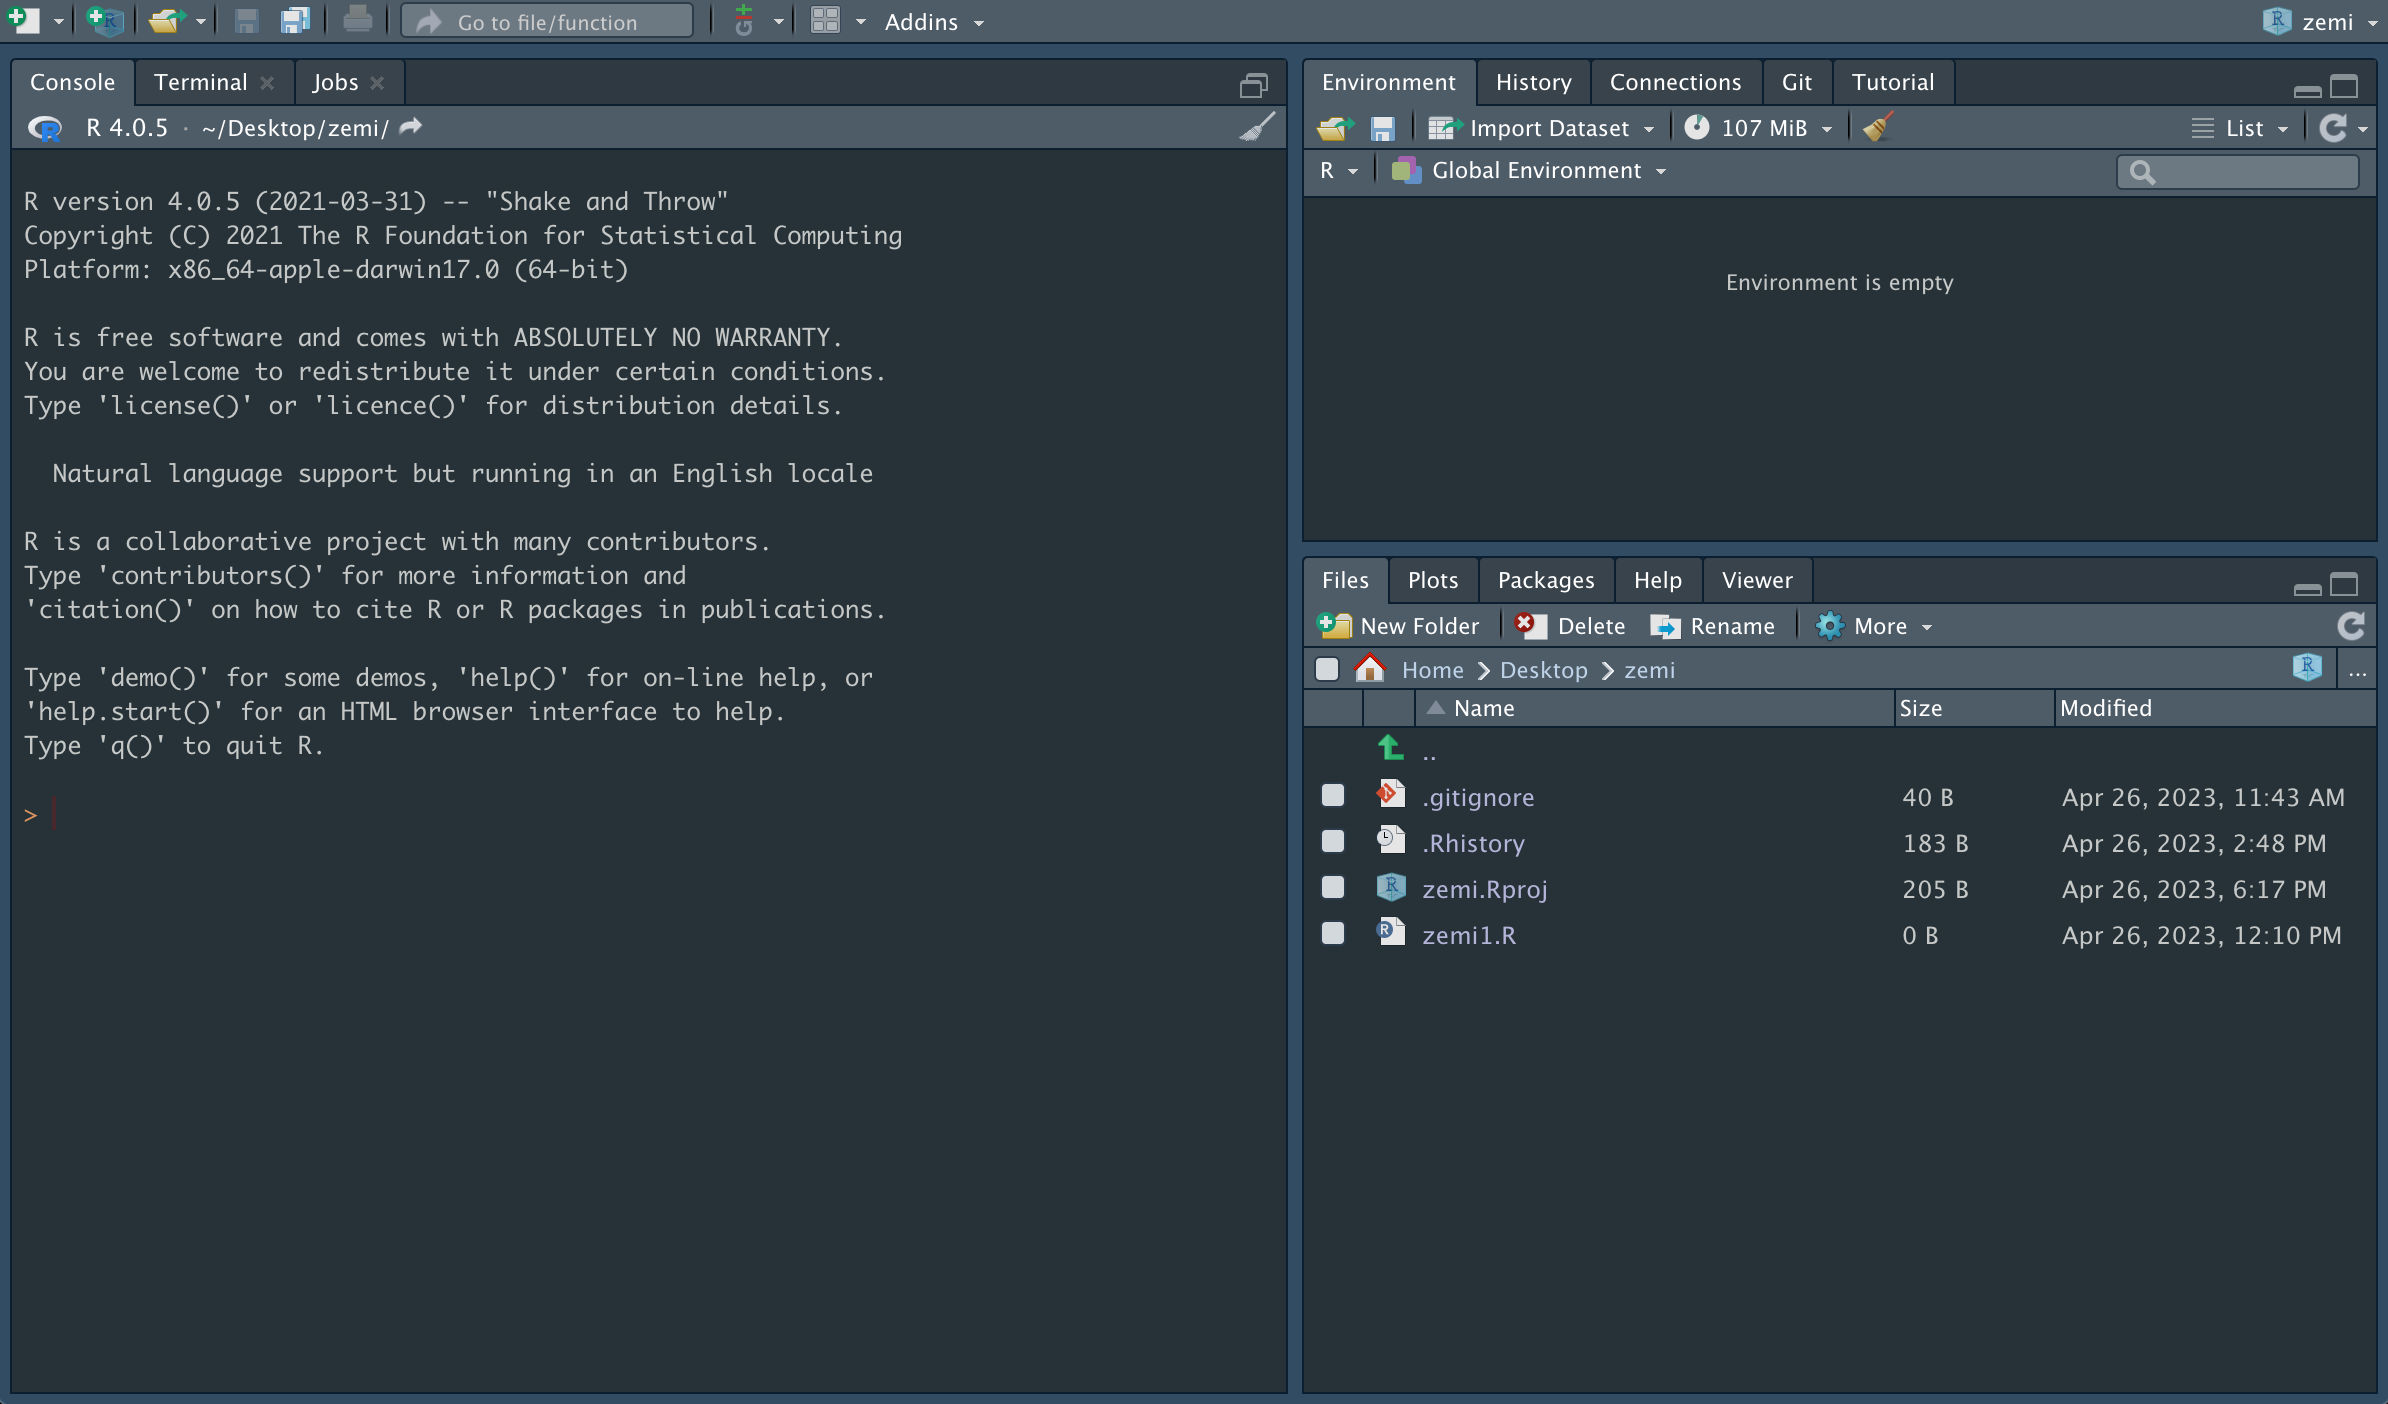
\includegraphics{./img/01_rstudio_start.png}
\end{itemize}

\begin{center}\rule{0.5\linewidth}{0.5pt}\end{center}

\hypertarget{ux30b3ux30f3ux30bdux30fcux30ebux306bux76f4ux63a5ux6253ux3061ux8fbcux3080}{%
\section{コンソールに直接打ち込む}\label{ux30b3ux30f3ux30bdux30fcux30ebux306bux76f4ux63a5ux6253ux3061ux8fbcux3080}}

\begin{itemize}
\tightlist
\item
  左側の大きな枠を見る\\
\item
  Consoleのタブが選択されていることを確認
\item
  この画面(=コンソール)を使い、簡単な足し算を実行しよう
\item
  最下段の\texttt{\textgreater{}}のあとに\texttt{1+1}と打ち込み\textbf{Enter(macはreturn)}を押す
\item
  \texttt{{[}1{]}\ 2}と返ってくる
\item
  \texttt{2}の部分が\texttt{1+1}の計算結果(\texttt{{[}1{]}}は1行目という意味)
\end{itemize}

\begin{center}\rule{0.5\linewidth}{0.5pt}\end{center}

\hypertarget{rux30b9ux30afux30eaux30d7ux30c8ux3092ux4f7fux3046}{%
\section{Rスクリプトを使う}\label{rux30b9ux30afux30eaux30d7ux30c8ux3092ux4f7fux3046}}

\begin{itemize}
\tightlist
\item
  コンソールに書いたコードは、Rstudioを終了すると消える\\
  (実際に終了して再起動してみよう)\\
\item
  だから、\textbf{Rスクリプト}と呼ばれる保存可能なファイルにコードを書くことが多い
\end{itemize}

\hypertarget{rux30b9ux30afux30eaux30d7ux30c8ux3092ux4f5cux308b}{%
\paragraph*{Rスクリプトを作る:}\label{rux30b9ux30afux30eaux30d7ux30c8ux3092ux4f5cux308b}}
\addcontentsline{toc}{paragraph}{Rスクリプトを作る:}

\begin{itemize}
\tightlist
\item
  RStudioの左上の
  をクリックし、「R Script」を選択
\item
  左上に新しくできた枠に、空のRスクリプトファイルが表示される\\
  (untitled1と表示されたタブが作成したRスクリプト)
\end{itemize}

\hypertarget{rstudioux306euxff14ux3064ux306eux30daux30fcux30f3}{%
\paragraph*{RStudioの4つのペーン:}\label{rstudioux306euxff14ux3064ux306eux30daux30fcux30f3}}
\addcontentsline{toc}{paragraph}{RStudioの4つのペーン:}

\begin{itemize}
\tightlist
\item
  実際には、この4つの枠(=ペーン)に分かれた画面で作業することが多い
\end{itemize}

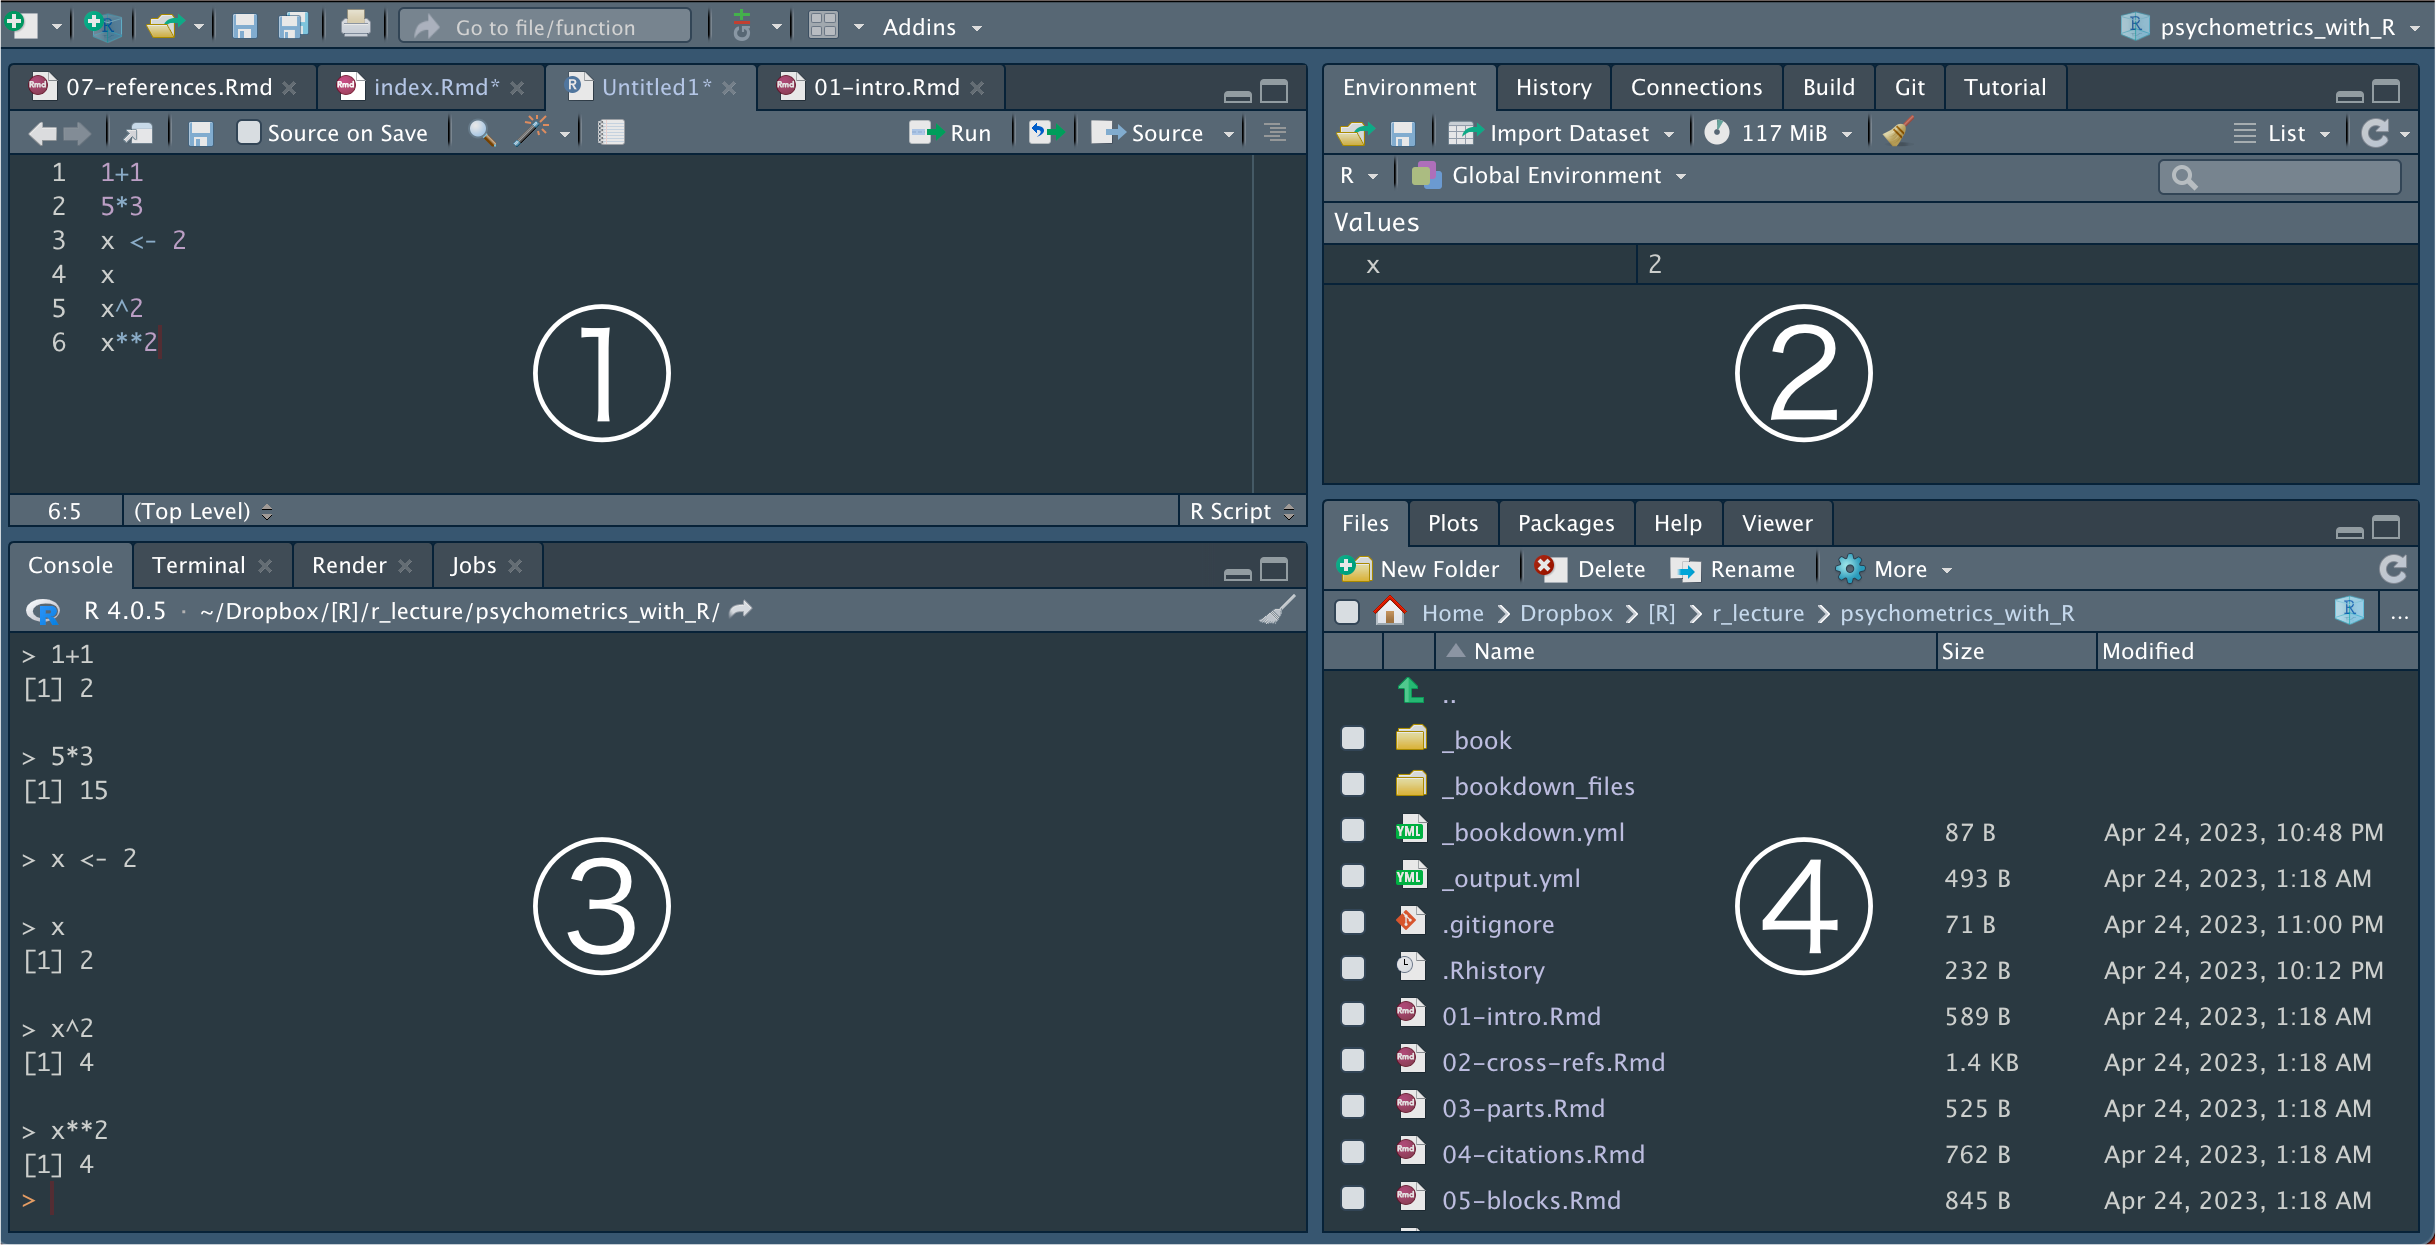
\includegraphics{./img/01_rstudio_4pane.png}

  \textbf{①左上:}メインの作業場で、Rスクリプトのコードなどを書くところ\\
  \textbf{②右上:}変数やオブジェクトのリストが表示されたり、バージョン管理を行う\\
  \textbf{③左下:}コードの実行結果が表示されるコンソールや、各種コマンドを実行するターミナルなど\\
  \textbf{④右下:}各種ファイルやパッケージの表示、出力した図の表示など

\hypertarget{rux30b9ux30afux30eaux30d7ux30c8ux306bux66f8ux304f}{%
\subsubsection*{Rスクリプトに書く:}\label{rux30b9ux30afux30eaux30d7ux30c8ux306bux66f8ux304f}}
\addcontentsline{toc}{subsubsection}{Rスクリプトに書く:}

\begin{itemize}
\tightlist
\item
  左上のペーンを見て、untitled1のタブが選択されていることを確認
\item
  1行目に\texttt{1+1}と入力して\textbf{ctrl+Enter(macはcommand+return)}を押す\\
  ( をクリックしても良い)
\item
  左下のペーンのコンソールに結果(\texttt{{[}1{]}\ 2})が表示される
\end{itemize}

\hypertarget{ux4fddux5b58}{%
\paragraph*{保存:}\label{ux4fddux5b58}}
\addcontentsline{toc}{paragraph}{保存:}

\begin{itemize}
\tightlist
\item
  Rスクリプトは\textbf{ctrl+s(macはcommand+s)}で好きな時に保存できる\\
  ( をクリックしても良い)
\item
  初回はファイル名と保存場所も決める
  (test.Rという名前でデスクトップに保存してみよう)
\item
  試しに、保存したRスクリプトのタブを閉じてみよう
  (test.Rのタブの右側の×をクリック)
\item
  左上の をクリックし、保存したRスクリプトのファイルを選択\\
  (つまり、デスクトップにあるtest.Rを選択)
\item
  Rスクリプトが先ほど保存した状態で開く
\end{itemize}

\hypertarget{ux3055ux3089ux306bux66f8ux304f}{%
\paragraph*{さらに書く!:}\label{ux3055ux3089ux306bux66f8ux304f}}
\addcontentsline{toc}{paragraph}{さらに書く!:}

\begin{itemize}
\tightlist
\item
  続けて、簡単な引き算を実行しよう
\item
  2行目に\texttt{5-2}と入力する
\item
  2行目にカーソルを合わせて\textbf{ctrl+Enter}を押す
\item
  2行目の計算結果(\texttt{{[}1{]}\ 3})が表示される
\item
  1行目にカーソルを合わせて\textbf{ctrl+Enter}を押す
\item
  1行目の計算結果(\texttt{{[}1{]}\ 2})が表示される
\item
  つまり、実行したい行にカーソルを合わせて\textbf{ctrl+Enter}を押せば良い
\item
  全ての行を一括で実行したいなら\textbf{ctrl+shift+Enter(macはcommand+shift+return)}
\item
  一部分だけ実行したいなら、下図のように実行したい行だけ選択して\textbf{ctrl+Enter}
\end{itemize}

\hypertarget{rux30b9ux30afux30eaux30d7ux30c8ux3092ux4f7fux3046ux30e1ux30eaux30c3ux30c8}{%
\paragraph*{Rスクリプトを使うメリット:}\label{rux30b9ux30afux30eaux30d7ux30c8ux3092ux4f7fux3046ux30e1ux30eaux30c3ux30c8}}
\addcontentsline{toc}{paragraph}{Rスクリプトを使うメリット:}

\begin{enumerate}
\def\labelenumi{\arabic{enumi}.}
\tightlist
\item
  コードが保存できる(毎回書き直さなくて良い!)
\item
  長く複雑なコードを書いたり、管理するのが楽\\
\item
  他の人に配布できる(分析を再現してもらいやすい)\\
  などなど\ldots{}
\end{enumerate}

\begin{center}\rule{0.5\linewidth}{0.5pt}\end{center}

\hypertarget{ux30d7ux30edux30b8ux30a7ux30afux30c8ux7ba1ux7406}{%
\section{プロジェクト管理}\label{ux30d7ux30edux30b8ux30a7ux30afux30c8ux7ba1ux7406}}

\begin{itemize}
\tightlist
\item
  研究プロジェクトが進むと、ひとつのRスクリプトだけでは管理しきれなくなる
\item
  \textbf{プロジェクト}を使えば、複数のRスクリプトや関連データなどを一つのフォルダにまとめて効率よく管理できる
\end{itemize}

\hypertarget{ux30d7ux30edux30b8ux30a7ux30afux30c8ux306eux4f5cux6210}{%
\paragraph*{プロジェクトの作成:}\label{ux30d7ux30edux30b8ux30a7ux30afux30c8ux306eux4f5cux6210}}
\addcontentsline{toc}{paragraph}{プロジェクトの作成:}

\begin{itemize}
\tightlist
\item
  左上の をクリックし、「New Directry」→「New Project」の順に選択\\
\item
  次の画面で①プロジェクト名と、その②作成場所を指定して③「Create Project」
\end{itemize}

\begin{itemize}
\tightlist
\item
  指定した場所に、指定したプロジェクト名のフォルダができているのを確認しよう\\
  (以降、これを\textbf{プロジェクトフォルダ}と呼ぶ)
\item
  そのフォルダの中に\texttt{プロジェクト名.Rproj}というファイルができているのを確認しよう
\item
  以下は、macで\texttt{Document}フォルダ内に\texttt{sugoi\_project}というプロジェクトを作った例
\end{itemize}

\begin{itemize}
\tightlist
\item
  初めはご利益がわかりにくいが、研究プロジェクトごとにプロジェクトを作るクセをつけよう
\item
  そして、次の心得に従い、プロジェクト上で作業をするようにしよう!
\end{itemize}

\begin{enumerate}
\def\labelenumi{\arabic{enumi}.}
\tightlist
\item
  毎回\texttt{プロジェクト名.Rproj}をダブルクリックしてRstudioを起動
\item
  関連するファイルはプロジェクトフォルダにまとめて一元管理
\end{enumerate}

\hypertarget{ux6f14ux7fd2ux554fux984c}{%
\section{演習問題}\label{ux6f14ux7fd2ux554fux984c}}

\begin{itemize}
\tightlist
\item
  自分の好きな場所に\texttt{zemi}という名前のプロジェクトを作る
\item
  指定した場所に\texttt{zemi}というフォルダができているのを確認する
\item
  フォルダの中に\texttt{zemi.Rproj}というファイルが出来ているのを確認
\end{itemize}

\textbf{※ 今後は、この\texttt{zemi}プロジェクトで作業していることを前提に解説する}

\hypertarget{ux57faux672cux64cdux4f5cux2460}{%
\chapter{基本操作①}\label{ux57faux672cux64cdux4f5cux2460}}

\begin{itemize}
\tightlist
\item
  本章の説明がわからない人は、森知晴先生のすばらしい動画たちを参考にしよう!
\end{itemize}

\begin{enumerate}
\def\labelenumi{\arabic{enumi}.}
\tightlist
\item
  \href{https://youtu.be/CblsIBlzqX0}{オブジェクトの使い方 in R}\\
\item
  \href{https://youtu.be/q8MI6P2hoUM}{関数の使い方 in R}
\end{enumerate}

\begin{itemize}
\tightlist
\item
  データ型やデータ構造については、逆瀬川浩孝先生のホームページを参照
\end{itemize}

  \href{http://www.f.waseda.jp/sakas/R/index.html}{「経営工学雑記帖」内のRのページ}

\hypertarget{ux56dbux5247ux6f14ux7b97}{%
\section{四則演算}\label{ux56dbux5247ux6f14ux7b97}}

\textbf{たし算:} \texttt{+}を使う

\begin{Shaded}
\begin{Highlighting}[]
\DecValTok{1} \SpecialCharTok{+} \DecValTok{1}
\end{Highlighting}
\end{Shaded}

\begin{verbatim}
## [1] 2
\end{verbatim}

\textbf{ひき算:} \texttt{-}を使う

\begin{Shaded}
\begin{Highlighting}[]
\DecValTok{5} \SpecialCharTok{{-}} \DecValTok{2}
\end{Highlighting}
\end{Shaded}

\begin{verbatim}
## [1] 3
\end{verbatim}

\textbf{かけ算:} \texttt{*}を使う

\begin{Shaded}
\begin{Highlighting}[]
\DecValTok{4} \SpecialCharTok{*} \DecValTok{5}
\end{Highlighting}
\end{Shaded}

\begin{verbatim}
## [1] 20
\end{verbatim}

\textbf{わり算:} \texttt{/}を使う(分数のイメージ)

\begin{Shaded}
\begin{Highlighting}[]
\DecValTok{8} \SpecialCharTok{/} \DecValTok{2}
\end{Highlighting}
\end{Shaded}

\begin{verbatim}
## [1] 4
\end{verbatim}

\textbf{累乗:} \texttt{\^{}}か\texttt{**}を使う(例:\(4^2\)なら次のとおり)

\begin{Shaded}
\begin{Highlighting}[]
\DecValTok{4} \SpecialCharTok{\^{}} \DecValTok{2}
\end{Highlighting}
\end{Shaded}

\begin{verbatim}
## [1] 16
\end{verbatim}

\begin{Shaded}
\begin{Highlighting}[]
\DecValTok{4} \SpecialCharTok{**} \DecValTok{2}
\end{Highlighting}
\end{Shaded}

\begin{verbatim}
## [1] 16
\end{verbatim}

\begin{itemize}
\tightlist
\item
  例えば、9÷2の答えは「4余り1」
\item
  この時、4を整数の商、1を剰余という
\end{itemize}

\textbf{整数の商:} \texttt{\%/\%}

\begin{Shaded}
\begin{Highlighting}[]
\DecValTok{9}\SpecialCharTok{\%/\%}\DecValTok{2}
\end{Highlighting}
\end{Shaded}

\begin{verbatim}
## [1] 4
\end{verbatim}

\textbf{剰余(mod):} \texttt{\%\%}

\begin{Shaded}
\begin{Highlighting}[]
\DecValTok{9}\SpecialCharTok{\%\%}\DecValTok{2}
\end{Highlighting}
\end{Shaded}

\begin{verbatim}
## [1] 1
\end{verbatim}

\begin{center}\rule{0.5\linewidth}{0.5pt}\end{center}

\hypertarget{ux5909ux6570ux30aaux30d6ux30b8ux30a7ux30afux30c8}{%
\section{変数(オブジェクト)}\label{ux5909ux6570ux30aaux30d6ux30b8ux30a7ux30afux30c8}}

\begin{itemize}
\item
  オブジェクトとは、色々なモノを入れる箱のようなもの\footnote{行列と同じ2次元のデータ構造だが、データフレームは列(変数)ごとに異なったデータ型を持てる}\\
\item
  オブジェクトを変数という人もいる(数学の変数のようなイメージだから)
\item
  本資料では変数と呼ぶことにする(字数が少ないから)
\item
  次のコードを見てみよう
\end{itemize}

\begin{Shaded}
\begin{Highlighting}[]
\NormalTok{x }\OtherTok{\textless{}{-}} \DecValTok{1} \CommentTok{\# \textless{}{-} は左向矢印のイメージ}

\CommentTok{\# このように\#から始まる文章を書いてコメントを残せる}
\CommentTok{\# これをコメントアウトと呼ぶ}
\CommentTok{\# あとで見てわかりやすいような覚え書きなどを残そう}
\end{Highlighting}
\end{Shaded}

\begin{itemize}
\tightlist
\item
  これはxという箱を作り、その中に数字の1を入れたイメージ\\
  (変数xに1を代入したイメージでもOK!)
\item
  上のコードを実行しても何も表示されないが、それでOK\\
  (「箱に入れる」だけのコードなので表示はされない)
\item
  変数の中身を確認したい時は、オブジェクトの名前を書いて実行
\end{itemize}

\begin{Shaded}
\begin{Highlighting}[]
\NormalTok{x}
\end{Highlighting}
\end{Shaded}

\begin{verbatim}
## [1] 1
\end{verbatim}

\begin{itemize}
\tightlist
\item
  数値を代入した変数同士で演算もできる
\end{itemize}

\begin{Shaded}
\begin{Highlighting}[]
\NormalTok{y }\OtherTok{\textless{}{-}} \DecValTok{1} 
\NormalTok{z }\OtherTok{\textless{}{-}} \DecValTok{2}
\NormalTok{y }\SpecialCharTok{*}\NormalTok{ z }\CommentTok{\# 1*2を計算したことになる}
\end{Highlighting}
\end{Shaded}

\begin{verbatim}
## [1] 2
\end{verbatim}

\begin{itemize}
\tightlist
\item
  変数はいつでも上書きできる
\end{itemize}

\begin{Shaded}
\begin{Highlighting}[]
\NormalTok{x }\OtherTok{\textless{}{-}} \DecValTok{1} \CommentTok{\#xに1を代入}
\NormalTok{x}
\end{Highlighting}
\end{Shaded}

\begin{verbatim}
## [1] 1
\end{verbatim}

\begin{Shaded}
\begin{Highlighting}[]
\NormalTok{x }\OtherTok{\textless{}{-}} \DecValTok{2} \CommentTok{\#xを2に上書き}
\NormalTok{x}
\end{Highlighting}
\end{Shaded}

\begin{verbatim}
## [1] 2
\end{verbatim}

\begin{itemize}
\tightlist
\item
  計算結果を変数に代入することもできる
\end{itemize}

\begin{Shaded}
\begin{Highlighting}[]
\NormalTok{x }\OtherTok{\textless{}{-}} \DecValTok{2}\SpecialCharTok{+}\DecValTok{5} 
\NormalTok{x }\CommentTok{\# 計算結果の7が代入される}
\end{Highlighting}
\end{Shaded}

\begin{verbatim}
## [1] 7
\end{verbatim}

\begin{itemize}
\tightlist
\item
  慣れるまでは不思議だが、こんなこともできる
\item
  意外とよく使うので、頭の片隅に留めておこう
\end{itemize}

\begin{Shaded}
\begin{Highlighting}[]
\NormalTok{suuji }\OtherTok{\textless{}{-}} \DecValTok{2} \CommentTok{\#suujiに2を代入}
\NormalTok{suuji }\OtherTok{\textless{}{-}}\NormalTok{ suuji }\SpecialCharTok{+} \DecValTok{1} \CommentTok{\#suuji=2に1を足したものを、もう一度suujiに代入}
\NormalTok{suuji }\CommentTok{\#新しいsuujiを表示}
\end{Highlighting}
\end{Shaded}

\begin{verbatim}
## [1] 3
\end{verbatim}

\begin{itemize}
\tightlist
\item
  変数には数値以外も入れることができる
\item
  例えば、mojiという変数を作り文字列を入れてみる
\end{itemize}

\begin{Shaded}
\begin{Highlighting}[]
\CommentTok{\# 文字列は"ダブルコーテーション"で囲む}
\CommentTok{\# \textquotesingle{}シングルコーテーション\textquotesingle{}でも良い}
\CommentTok{\# 次のようにアルファベット以外も一応使えるが推奨しない}

\NormalTok{moji }\OtherTok{\textless{}{-}} \StringTok{"岡田先生ステキ"}
\NormalTok{moji}
\end{Highlighting}
\end{Shaded}

\begin{verbatim}
## [1] "岡田先生ステキ"
\end{verbatim}

\hypertarget{ux7df4ux7fd2ux554fux984c}{%
\paragraph*{練習問題}\label{ux7df4ux7fd2ux554fux984c}}
\addcontentsline{toc}{paragraph}{練習問題}

\begin{itemize}
\tightlist
\item
  変数xに3、変数yに6を代入する
\item
  xとyをそれぞれ2乗して和をとり、結果が45となることを確認する
\end{itemize}

\begin{center}\rule{0.5\linewidth}{0.5pt}\end{center}

\hypertarget{ux95a2ux6570ux2460ux6570ux5024ux306bux5bfeux3059ux308bux95a2ux6570}{%
\section{関数①(数値に対する関数)}\label{ux95a2ux6570ux2460ux6570ux5024ux306bux5bfeux3059ux308bux95a2ux6570}}

\hypertarget{ux95a2ux6570ux306eux30adux30dbux30f3}{%
\subsubsection*{関数のキホン:}\label{ux95a2ux6570ux306eux30adux30dbux30f3}}
\addcontentsline{toc}{subsubsection}{関数のキホン:}

\begin{itemize}
\tightlist
\item
  Rにはさまざまな機能を実行できる関数が用意されている
\item
  例えば、平方根を計算する関数が\texttt{sqrt()}
\item
  \texttt{()}の中に数値を入れると、その平方根を返してくれる
\end{itemize}

\begin{Shaded}
\begin{Highlighting}[]
\FunctionTok{sqrt}\NormalTok{(}\DecValTok{2}\NormalTok{)}
\end{Highlighting}
\end{Shaded}

\begin{verbatim}
## [1] 1.414214
\end{verbatim}

\begin{itemize}
\tightlist
\item
  このように関数は\texttt{xxx()}のように最後が丸括弧になっている
\item
  丸括弧の中に、引数(ひきすう)と呼ばれる指定された形式の値を入れて実行する
\item
  その結果、出力された値を戻り値という
\item
  先ほどの\texttt{sqrt(2)}なら\texttt{2}が引数で、計算結果の\texttt{1.414214}が戻り値
\end{itemize}

\hypertarget{ux8907ux6570ux306eux5f15ux6570ux3092ux6301ux3064ux95a2ux6570}{%
\subsubsection*{複数の引数を持つ関数:}\label{ux8907ux6570ux306eux5f15ux6570ux3092ux6301ux3064ux95a2ux6570}}
\addcontentsline{toc}{subsubsection}{複数の引数を持つ関数:}

\begin{itemize}
\tightlist
\item
  引数は1つとは限らないので注意
\item
  例えば、\texttt{log()}は対数を計算する関数
\item
  次のようにすると、10の自然対数を返してくれる
\end{itemize}

\begin{Shaded}
\begin{Highlighting}[]
\FunctionTok{log}\NormalTok{(}\DecValTok{10}\NormalTok{)}
\end{Highlighting}
\end{Shaded}

\begin{verbatim}
## [1] 2.302585
\end{verbatim}

\begin{itemize}
\tightlist
\item
  でも、2つ目の引数\texttt{base=10}を付け足すと、底が10の常用対数を返してくれる
\end{itemize}

\begin{Shaded}
\begin{Highlighting}[]
\FunctionTok{log}\NormalTok{(}\DecValTok{10}\NormalTok{, }\AttributeTok{base =} \DecValTok{10}\NormalTok{)}
\end{Highlighting}
\end{Shaded}

\begin{verbatim}
## [1] 1
\end{verbatim}

\begin{itemize}
\tightlist
\item
  数値(numeric型)を引数にする関数のうち、よく使うものを列挙する
\end{itemize}

\begin{longtable}[]{@{}
  >{\raggedright\arraybackslash}p{(\columnwidth - 2\tabcolsep) * \real{0.5000}}
  >{\raggedright\arraybackslash}p{(\columnwidth - 2\tabcolsep) * \real{0.5000}}@{}}
\toprule()
\begin{minipage}[b]{\linewidth}\raggedright
関数(引数xは数値)
\end{minipage} & \begin{minipage}[b]{\linewidth}\raggedright
意味
\end{minipage} \\
\midrule()
\endhead
log(x) & 自然対数 \\
log(x, base=y) & yを底とする常用対数 \\
sqrt(x) & xの平方根 \\
exp(x) & x指数関数(\(e^x\))) \\
abs(x) & xの絶対値 \\
round(x,y) & 小数点以下y桁になるようxを四捨五入(IEEE754方式)※ 詳細は演習問題参照 \\
floor(x) & xの小数点以下切り捨て \\
ceiling(x) & xの小数点以下切り上げ \\
\bottomrule()
\end{longtable}

\begin{itemize}
\tightlist
\item
  他にも、数え切れないほどの関数がある
\end{itemize}

\hypertarget{ux95a2ux6570ux306eux6a5fux80fdux3084ux5f15ux6570ux306eux8abfux3079ux65b9}{%
\subsubsection*{関数の機能や引数の調べ方:}\label{ux95a2ux6570ux306eux6a5fux80fdux3084ux5f15ux6570ux306eux8abfux3079ux65b9}}
\addcontentsline{toc}{subsubsection}{関数の機能や引数の調べ方:}

\begin{itemize}
\tightlist
\item
  関数の機能や、どんな形式の引数をいくつ持つかを調べるには\texttt{help()}を使う
\item
  知りたい関数から\texttt{()}を除いたものを、\texttt{help()}の中に入れる
\item
  例えば、\texttt{log()}について知りたいなら\texttt{help(log)}と書いて実行
\item
  すると、Rstudioの右下(左下ではない!)のペーンに詳細が表示される
\end{itemize}

\begin{center}\rule{0.5\linewidth}{0.5pt}\end{center}

\hypertarget{ux30c7ux30fcux30bfux578bux306eux30adux30dbux30f3}{%
\section{データ型のキホン}\label{ux30c7ux30fcux30bfux578bux306eux30adux30dbux30f3}}

\begin{itemize}
\tightlist
\item
  次の2つの変数に対して\texttt{+\ 1}という演算を実行してみよう
\end{itemize}

\begin{Shaded}
\begin{Highlighting}[]
\NormalTok{suuji }\OtherTok{\textless{}{-}} \DecValTok{2} 
\NormalTok{suuji }\SpecialCharTok{+} \DecValTok{1} 

\NormalTok{moji }\OtherTok{\textless{}{-}} \StringTok{"岡田先生ステキ"}
\NormalTok{moji }\SpecialCharTok{+} \DecValTok{1}
\end{Highlighting}
\end{Shaded}

\begin{itemize}
\tightlist
\item
  ひとつ目は\texttt{3}という結果を得るが、ふたつ目はエラーが出て処理できない
\item
  この理由を考えてみよう
\item
  \texttt{suuji}に格納された\texttt{2}というデータは、数字の型(\texttt{numeric}ないし\texttt{double})を持っている\\
\item
  \texttt{moji}に格納された文字列のデータは、文字列の型(\texttt{character})を持っている\\
\item
  \texttt{character}型のデータに対しては、\texttt{+}を使った演算が定義されていないからエラーが出た\\
\item
  このように、\texttt{+}のような演算子や関数は、特定のデータ型に対してしか使えない
\item
  データ型を確認するには\texttt{typeof()}か\texttt{mode()}の関数を使う
\end{itemize}

\begin{Shaded}
\begin{Highlighting}[]
\FunctionTok{typeof}\NormalTok{(suuji)}
\end{Highlighting}
\end{Shaded}

\begin{verbatim}
## [1] "double"
\end{verbatim}

\begin{Shaded}
\begin{Highlighting}[]
\FunctionTok{typeof}\NormalTok{(moji)}
\end{Highlighting}
\end{Shaded}

\begin{verbatim}
## [1] "character"
\end{verbatim}

\begin{itemize}
\tightlist
\item
  他によく使うデータ型には真偽値(TRUEとFALSE)をあつかう\texttt{logical}がある
\item
  データ型についての詳しい説明は\href{http://www.f.waseda.jp/sakas/R/Rdata.html}{逆瀬川先生のホームページ内のコチラ}を参照
\end{itemize}

\hypertarget{ux7df4ux7fd2ux554fux984c-1}{%
\paragraph*{練習問題}\label{ux7df4ux7fd2ux554fux984c-1}}
\addcontentsline{toc}{paragraph}{練習問題}

\begin{itemize}
\tightlist
\item
  上の\texttt{suuji}と\texttt{moji}について、\texttt{mode(suuji)}と\texttt{mode(moji)}を実行する
\item
  \texttt{typeof(suuji)}と\texttt{mode(suuji)}の結果を比較する
\end{itemize}

\begin{center}\rule{0.5\linewidth}{0.5pt}\end{center}

\hypertarget{ux6f14ux7fd2ux554fux984c-1}{%
\section{演習問題}\label{ux6f14ux7fd2ux554fux984c-1}}

\begin{itemize}
\tightlist
\item
  \texttt{zemi}という名前のプロジェクトの中に、\texttt{exercise\_ch3.R}というRスクリプトを作りなさい
\item
  \texttt{exercise\_ch3.R}に、以下の問題に答るためのコードを書きなさい
\end{itemize}

\begin{enumerate}
\def\labelenumi{\arabic{enumi}.}
\tightlist
\item
  \texttt{abs(-5)}の結果を確認する
\item
  \texttt{x\ \textless{}-\ exp(10)}とした上で、\texttt{log(x)}の結果を確認
\end{enumerate}

\textbf{挑戦問題:}

\begin{enumerate}
\def\labelenumi{\arabic{enumi}.}
\tightlist
\item
  \texttt{round(0.45,\ 1)}が\texttt{0.5}ではなく\texttt{0.4}になることを確認する\\
  (IEEE式の四捨五入では、末尾が偶数になるように5を丸める)
\item
  \texttt{floor(0.45\ *\ 10)/10}で、通常の四捨五入(\texttt{0.5})になることを確認する\\
  (xに対し、小数点以下y桁となるように通常の四捨五入をするには\texttt{floor(x\ *\ 10\^{}y\ +\ 0.5)/10\^{}y})
\end{enumerate}

\hypertarget{ux57faux672cux64cdux4f5cux2461}{%
\chapter{基本操作②}\label{ux57faux672cux64cdux4f5cux2461}}

\begin{itemize}
\tightlist
\item
  本章の説明がわからない人は、森知晴先生のすばらしい動画たちを参考にしよう!
\end{itemize}

\begin{enumerate}
\def\labelenumi{\arabic{enumi}.}
\tightlist
\item
  \href{https://youtu.be/CblsIBlzqX0}{オブジェクトの使い方 in R}\\
\item
  \href{https://youtu.be/q8MI6P2hoUM}{関数の使い方 in R}
\end{enumerate}

\begin{itemize}
\tightlist
\item
  データ型やデータ構造については、逆瀬川浩孝先生のホームページを参照
\end{itemize}

  \href{http://www.f.waseda.jp/sakas/R/index.html}{「経営工学雑記帖」内のRのページ}

\hypertarget{ux30d9ux30afux30c8ux30ebux3068ux884cux5217}{%
\section{ベクトルと行列}\label{ux30d9ux30afux30c8ux30ebux3068ux884cux5217}}

\begin{itemize}
\tightlist
\item
  Rでは、複数のデータの値をひとまとめにして扱いやすくできる
\end{itemize}

\hypertarget{ux30d9ux30afux30c8ux30eb}{%
\subsection{ベクトル}\label{ux30d9ux30afux30c8ux30eb}}

\begin{itemize}
\tightlist
\item
  同じ型のデータを1列に並べたものをベクトルと呼ぶ
\item
  ベクトルは関数\texttt{c()}を使って作る
\item
  ベクトルも変数に入れることができる
\item
  例として、5つの数字(例えば、2,4,2,3,5)を並べたベクトルを変数\texttt{v}に代入する
\end{itemize}

\begin{Shaded}
\begin{Highlighting}[]
\NormalTok{v }\OtherTok{\textless{}{-}} \FunctionTok{c}\NormalTok{(}\DecValTok{2}\NormalTok{, }\DecValTok{4}\NormalTok{, }\DecValTok{2}\NormalTok{, }\DecValTok{3}\NormalTok{, }\DecValTok{5}\NormalTok{) }\CommentTok{\#ベクトルを作り変数に代入}
\NormalTok{v }\CommentTok{\#変数vの中身を確認}
\end{Highlighting}
\end{Shaded}

\begin{verbatim}
## [1] 2 4 2 3 5
\end{verbatim}

\begin{itemize}
\tightlist
\item
  連番のベクトル(例えば2,3,4,5,6)を作りたい時は、次のようにも書ける
\end{itemize}

\begin{Shaded}
\begin{Highlighting}[]
\NormalTok{v2\_6 }\OtherTok{\textless{}{-}} \FunctionTok{c}\NormalTok{(}\DecValTok{2}\SpecialCharTok{:}\DecValTok{6}\NormalTok{) }\CommentTok{\#「n:m」で「nからmまで」の意味}
\NormalTok{v2\_6}
\end{Highlighting}
\end{Shaded}

\begin{verbatim}
## [1] 2 3 4 5 6
\end{verbatim}

\hypertarget{ux30d9ux30afux30c8ux30ebux3068ux6570ux5024ux306eux6f14ux7b97}{%
\subsubsection*{ベクトルと数値の演算:}\label{ux30d9ux30afux30c8ux30ebux3068ux6570ux5024ux306eux6f14ux7b97}}
\addcontentsline{toc}{subsubsection}{ベクトルと数値の演算:}

\begin{itemize}
\tightlist
\item
  ベクトルにも四則演算の記号(=演算子)を使った演算ができる
\item
  ベクトル内のそれぞれの数字に、四則演算が施される
\item
  以下の出力結果で確認してみよう
\end{itemize}

\begin{Shaded}
\begin{Highlighting}[]
\NormalTok{v}
\end{Highlighting}
\end{Shaded}

\begin{verbatim}
## [1] 2 4 2 3 5
\end{verbatim}

\begin{Shaded}
\begin{Highlighting}[]
\NormalTok{v}\SpecialCharTok{+}\DecValTok{2}  \CommentTok{\#それぞれの数字に2を足す }
\end{Highlighting}
\end{Shaded}

\begin{verbatim}
## [1] 4 6 4 5 7
\end{verbatim}

\begin{Shaded}
\begin{Highlighting}[]
\DecValTok{2}\SpecialCharTok{*}\NormalTok{v  }\CommentTok{\#それぞれの数字に2をかける  }
\end{Highlighting}
\end{Shaded}

\begin{verbatim}
## [1]  4  8  4  6 10
\end{verbatim}

\hypertarget{ux7df4ux7fd2ux554fux984c-2}{%
\paragraph*{練習問題}\label{ux7df4ux7fd2ux554fux984c-2}}
\addcontentsline{toc}{paragraph}{練習問題}

\begin{itemize}
\tightlist
\item
  上の\texttt{v}について、\texttt{v-2}、\texttt{v/2}、\texttt{v\^{}2}の実行結果を確認する
\end{itemize}

\hypertarget{ux30d9ux30afux30c8ux30ebux540cux58ebux306eux6f14ux7b97}{%
\subsubsection*{ベクトル同士の演算:}\label{ux30d9ux30afux30c8ux30ebux540cux58ebux306eux6f14ux7b97}}
\addcontentsline{toc}{subsubsection}{ベクトル同士の演算:}

\begin{itemize}
\tightlist
\item
  Rでは、ベクトル同士の演算もできる
\item
  まずは2つのベクトルを用意しよう
\end{itemize}

\begin{Shaded}
\begin{Highlighting}[]
\NormalTok{v1 }\OtherTok{\textless{}{-}} \FunctionTok{c}\NormalTok{(}\DecValTok{1}\NormalTok{, }\DecValTok{2}\NormalTok{) }
\NormalTok{v2 }\OtherTok{\textless{}{-}} \FunctionTok{c}\NormalTok{(}\DecValTok{2}\NormalTok{, }\DecValTok{4}\NormalTok{) }
\end{Highlighting}
\end{Shaded}

\begin{itemize}
\tightlist
\item
  これらを\texttt{+}を使って「足す」
\item
  すると、1つめの数同士(1と2)と、2つめの数同士(2と4)が足される
\end{itemize}

\begin{Shaded}
\begin{Highlighting}[]
\NormalTok{v1 }\SpecialCharTok{+}\NormalTok{ v2}
\end{Highlighting}
\end{Shaded}

\begin{verbatim}
## [1] 3 6
\end{verbatim}

\begin{itemize}
\tightlist
\item
  \texttt{*}を使って「かける」場合も、同じように1つめの数同士、2つめの数同士がかけられる
\end{itemize}

\begin{Shaded}
\begin{Highlighting}[]
\NormalTok{v1 }\SpecialCharTok{*}\NormalTok{ v2}
\end{Highlighting}
\end{Shaded}

\begin{verbatim}
## [1] 2 8
\end{verbatim}

\begin{itemize}
\tightlist
\item
  ベクトル同士の「かけ算」には内積がある
\item
  Rでは、\texttt{\%*\%}で内積を計算できる
\end{itemize}

\begin{Shaded}
\begin{Highlighting}[]
\NormalTok{v1 }\SpecialCharTok{\%*\%}\NormalTok{ v2 }
\end{Highlighting}
\end{Shaded}

\begin{verbatim}
##      [,1]
## [1,]   10
\end{verbatim}

\begin{itemize}
\tightlist
\item
  ベクトルの長さ(=入っている数値の個数)が違うとおかしな計算になり、警告が出る
\end{itemize}

\begin{Shaded}
\begin{Highlighting}[]
\CommentTok{\#以下のv1には3つの要素があるけど、v2には2つしかない}
\CommentTok{\#この場合、v2の1つめの要素を無理やりv1の3つめに足してしまう}

\NormalTok{v1 }\OtherTok{\textless{}{-}} \FunctionTok{c}\NormalTok{(}\DecValTok{1}\NormalTok{, }\DecValTok{2}\NormalTok{, }\DecValTok{3}\NormalTok{)  }\CommentTok{\#3つの数を代入}
\NormalTok{v2 }\OtherTok{\textless{}{-}} \FunctionTok{c}\NormalTok{(}\DecValTok{2}\NormalTok{, }\DecValTok{4}\NormalTok{) }\CommentTok{\#2つの数を代入}
\NormalTok{v1 }\SpecialCharTok{+}\NormalTok{ v2 }\CommentTok{\#長さが違うからうまく計算できず警告が出る}
\end{Highlighting}
\end{Shaded}

\begin{verbatim}
## Warning in v1 + v2: longer object length is not a multiple of shorter object
## length
\end{verbatim}

\begin{verbatim}
## [1] 3 6 5
\end{verbatim}

\begin{itemize}
\tightlist
\item
  ベクトルの長さを確認するには\texttt{length()}を使えば良い
\end{itemize}

\begin{Shaded}
\begin{Highlighting}[]
\FunctionTok{length}\NormalTok{(v1)}
\end{Highlighting}
\end{Shaded}

\begin{verbatim}
## [1] 3
\end{verbatim}

\hypertarget{ux7df4ux7fd2ux554fux984c-3}{%
\paragraph*{練習問題}\label{ux7df4ux7fd2ux554fux984c-3}}
\addcontentsline{toc}{paragraph}{練習問題}

\begin{itemize}
\tightlist
\item
  上の\texttt{v1}と\texttt{v2}を使い、\texttt{-}、\texttt{/}、\texttt{\^{}}の3つの演算を行う
\item
  いずれも1つめの数値同士、2つめの数値同士で対応した演算がなされることを確かめる
\end{itemize}

\hypertarget{ux8981ux7d20ux306eux62bdux51fa}{%
\subsubsection*{要素の抽出:}\label{ux8981ux7d20ux306eux62bdux51fa}}
\addcontentsline{toc}{subsubsection}{要素の抽出:}

\begin{itemize}
\item
  ベクトルから、任意の要素(\texttt{n}番目の数)を抽出する方法を説明する
\item
  \texttt{x}という名前のベクトルからn番目の要素を抽出する時は\texttt{x{[}n{]}}
\item
  具体例として、先ほどのベクトル\texttt{v=c(2,4,2,3,5)}で考える
\item
  2番目の要素(つまり4)を抜き出したいなら、\texttt{v{[}2{]}}と書く
\item
  2〜4番めの要素(つまり4,2,3)を抜き出したいなら、\texttt{v{[}2:4{]}}と書く
\end{itemize}

\begin{Shaded}
\begin{Highlighting}[]
\NormalTok{v[}\DecValTok{2}\SpecialCharTok{:}\DecValTok{4}\NormalTok{]}
\end{Highlighting}
\end{Shaded}

\begin{verbatim}
## [1] 4 2 3
\end{verbatim}

\hypertarget{ux884cux5217}{%
\subsection{行列}\label{ux884cux5217}}

\hypertarget{ux884cux5217ux306eux30adux30dbux30f3}{%
\subsubsection*{行列のキホン:}\label{ux884cux5217ux306eux30adux30dbux30f3}}
\addcontentsline{toc}{subsubsection}{行列のキホン:}

\begin{itemize}
\tightlist
\item
  同じ型のデータを行と列の2次元に並べたものを行列と呼ぶ
\item
  例えば、2行3列の行列
  \(\begin{pmatrix} 1 & 2 & 3 \\ 4 & 5 & 6 \\ \end{pmatrix}\)
  を作ってMに代入するには、\texttt{matrix()}を使い次のように書く
\end{itemize}

\begin{Shaded}
\begin{Highlighting}[]
\CommentTok{\#初めの1:6はc(1:6)と同じで「1,2,3,4,5,6」の意味}
\CommentTok{\#この6つの数字を、2つの行(row)と3つの列(col)に分ける}
\CommentTok{\#byrow = Tで、6つの数字を左から右(zの書き順)に埋めるよう指示}
\CommentTok{\#byrow = Tを消すと、上から下に埋める(各自確かめよう)}

\NormalTok{M }\OtherTok{\textless{}{-}} \FunctionTok{matrix}\NormalTok{(}\DecValTok{1}\SpecialCharTok{:}\DecValTok{6}\NormalTok{, }\AttributeTok{nrow =} \DecValTok{2}\NormalTok{, }\AttributeTok{ncol =} \DecValTok{3}\NormalTok{, }\AttributeTok{byrow =}\NormalTok{ T)}
\NormalTok{M}
\end{Highlighting}
\end{Shaded}

\begin{verbatim}
##      [,1] [,2] [,3]
## [1,]    1    2    3
## [2,]    4    5    6
\end{verbatim}

\begin{itemize}
\tightlist
\item
  次の関数を使って、ベクトル同士を結合しても行列を作れる
\end{itemize}

\begin{Shaded}
\begin{Highlighting}[]
\NormalTok{v1 }\OtherTok{\textless{}{-}} \FunctionTok{c}\NormalTok{(}\DecValTok{1}\NormalTok{,}\DecValTok{2}\NormalTok{,}\DecValTok{3}\NormalTok{) }
\NormalTok{v2 }\OtherTok{\textless{}{-}} \FunctionTok{c}\NormalTok{(}\DecValTok{1}\NormalTok{,}\DecValTok{1}\NormalTok{,}\DecValTok{1}\NormalTok{) }\CommentTok{\#2つのベクトルv1とv2を作る}

\FunctionTok{rbind}\NormalTok{(v1, v2) }\CommentTok{\#v1とv2を行(row)方向に繋げる}
\end{Highlighting}
\end{Shaded}

\begin{verbatim}
##    [,1] [,2] [,3]
## v1    1    2    3
## v2    1    1    1
\end{verbatim}

\begin{Shaded}
\begin{Highlighting}[]
\FunctionTok{cbind}\NormalTok{(v1, v2) }\CommentTok{\#v1とv2を列(column)方向に繋げる}
\end{Highlighting}
\end{Shaded}

\begin{verbatim}
##      v1 v2
## [1,]  1  1
## [2,]  2  1
## [3,]  3  1
\end{verbatim}

\begin{Shaded}
\begin{Highlighting}[]
\FunctionTok{rbind}\NormalTok{(M, v1) }\CommentTok{\#「行列とベクトル」や「行列同士」も繋げられる}
\end{Highlighting}
\end{Shaded}

\begin{verbatim}
##    [,1] [,2] [,3]
##       1    2    3
##       4    5    6
## v1    1    2    3
\end{verbatim}

\hypertarget{ux8981ux7d20ux306eux62bdux51fa-1}{%
\subsubsection*{要素の抽出:}\label{ux8981ux7d20ux306eux62bdux51fa-1}}
\addcontentsline{toc}{subsubsection}{要素の抽出:}

\begin{itemize}
\tightlist
\item
  行列\texttt{x}から要素を抜き出すには、\texttt{x{[}抜き出したい行、抜き出したい列{]}}と書く
\item
  具体例として、先の行列\texttt{M}から色々な要素を抜き出してみよう
\end{itemize}

\begin{Shaded}
\begin{Highlighting}[]
\CommentTok{\# 2行1列目を抽出し、変数M21に代入}
\NormalTok{M21 }\OtherTok{\textless{}{-}}\NormalTok{ M[}\DecValTok{2}\NormalTok{,}\DecValTok{1}\NormalTok{]}

\CommentTok{\# 2行めを抽出}
\NormalTok{M[}\DecValTok{2}\NormalTok{,]}
\end{Highlighting}
\end{Shaded}

\begin{verbatim}
## [1] 4 5 6
\end{verbatim}

\begin{Shaded}
\begin{Highlighting}[]
\CommentTok{\# 1列めを抽出}
\NormalTok{M[,}\DecValTok{1}\NormalTok{]}
\end{Highlighting}
\end{Shaded}

\begin{verbatim}
## [1] 1 4
\end{verbatim}

\begin{Shaded}
\begin{Highlighting}[]
\CommentTok{\# 1,2行めと1,3列めを抽出}
\NormalTok{M[}\FunctionTok{c}\NormalTok{(}\DecValTok{1}\NormalTok{,}\DecValTok{2}\NormalTok{),}\FunctionTok{c}\NormalTok{(}\DecValTok{1}\NormalTok{,}\DecValTok{3}\NormalTok{)]}
\end{Highlighting}
\end{Shaded}

\begin{verbatim}
##      [,1] [,2]
## [1,]    1    3
## [2,]    4    6
\end{verbatim}

\hypertarget{ux884cux5217ux306eux6f14ux7b97}{%
\subsubsection*{行列の演算:}\label{ux884cux5217ux306eux6f14ux7b97}}
\addcontentsline{toc}{subsubsection}{行列の演算:}

\begin{itemize}
\tightlist
\item
  n行n列の2つの行列同士の計算について、足し算は\texttt{+}、引き算は\texttt{-}を使えば良い
\item
  以下の例のように、かけ算は\texttt{\%*\%}を使わなくてはいけないので注意
\end{itemize}

\begin{Shaded}
\begin{Highlighting}[]
\NormalTok{M }\CommentTok{\#先ほど作った2行3列の行列を表示}
\end{Highlighting}
\end{Shaded}

\begin{verbatim}
##      [,1] [,2] [,3]
## [1,]    1    2    3
## [2,]    4    5    6
\end{verbatim}

\begin{Shaded}
\begin{Highlighting}[]
\NormalTok{M2 }\OtherTok{\textless{}{-}} \FunctionTok{matrix}\NormalTok{(}\FunctionTok{c}\NormalTok{(}\DecValTok{1}\NormalTok{,}\DecValTok{2}\NormalTok{,}\DecValTok{0}\NormalTok{,}\DecValTok{1}\NormalTok{,}\DecValTok{0}\NormalTok{,}\DecValTok{2}\NormalTok{), }\AttributeTok{nrow =} \DecValTok{3}\NormalTok{, }\AttributeTok{ncol =} \DecValTok{2}\NormalTok{, }\AttributeTok{byrow =}\NormalTok{ T) }\CommentTok{\#新たに3行2列の行列を作る}
\NormalTok{M2 }\CommentTok{\#今作った2行3列の行列を表示}
\end{Highlighting}
\end{Shaded}

\begin{verbatim}
##      [,1] [,2]
## [1,]    1    2
## [2,]    0    1
## [3,]    0    2
\end{verbatim}

\begin{Shaded}
\begin{Highlighting}[]
\CommentTok{\#2つの行列の積MN}
\NormalTok{M }\SpecialCharTok{\%*\%}\NormalTok{ M2 }
\end{Highlighting}
\end{Shaded}

\begin{verbatim}
##      [,1] [,2]
## [1,]    1   10
## [2,]    4   25
\end{verbatim}

\begin{Shaded}
\begin{Highlighting}[]
\CommentTok{\#2つの行列の積MN}
\NormalTok{M2 }\SpecialCharTok{\%*\%}\NormalTok{ M }
\end{Highlighting}
\end{Shaded}

\begin{verbatim}
##      [,1] [,2] [,3]
## [1,]    9   12   15
## [2,]    4    5    6
## [3,]    8   10   12
\end{verbatim}

\begin{Shaded}
\begin{Highlighting}[]
\NormalTok{v }\OtherTok{\textless{}{-}} \FunctionTok{c}\NormalTok{(}\DecValTok{1}\NormalTok{,}\DecValTok{2}\NormalTok{,}\DecValTok{3}\NormalTok{) }\CommentTok{\#要素が3つのベクトルを作る}

\CommentTok{\#行列とベクトルのかけ算も\%*\%を使う}
\CommentTok{\#縦ベクトルと横ベクトルは区別されないので、次のコードで計算できる}
\NormalTok{v }\SpecialCharTok{\%*\%}\NormalTok{ M2 }\CommentTok{\# ただし、M2\%*\%vのように計算できない場合はエラーが出る(各自確かめよう)}
\end{Highlighting}
\end{Shaded}

\begin{verbatim}
##      [,1] [,2]
## [1,]    1   10
\end{verbatim}

\begin{center}\rule{0.5\linewidth}{0.5pt}\end{center}

\hypertarget{ux95a2ux6570ux2461ux30d9ux30afux30c8ux30ebux3084ux884cux5217ux306bux5bfeux3059ux308bux95a2ux6570}{%
\section{関数②(ベクトルや行列に対する関数)}\label{ux95a2ux6570ux2461ux30d9ux30afux30c8ux30ebux3084ux884cux5217ux306bux5bfeux3059ux308bux95a2ux6570}}

\begin{itemize}
\tightlist
\item
  先の\texttt{rbind()}や\texttt{cbind()}はベクトルや行列も引数にとれる関数だった
\item
  ベクトルや行列に対して使える他の関数をいくつか紹介する
\end{itemize}

\hypertarget{ux30d9ux30afux30c8ux30ebux306eux983bux51faux95a2ux6570}{%
\subsubsection*{ベクトルの頻出関数:}\label{ux30d9ux30afux30c8ux30ebux306eux983bux51faux95a2ux6570}}
\addcontentsline{toc}{subsubsection}{ベクトルの頻出関数:}

\begin{itemize}
\tightlist
\item
  以下の関数はどれもよく使うので、しっかり覚えよう
\end{itemize}

\begin{longtable}[]{@{}ll@{}}
\toprule()
関数(引数xはベクトル) & 意味 \\
\midrule()
\endhead
summary(x) & 基本統計量の一括表示 \\
max(x) & xの要素の最大値 \\
min(x) & xの要素の最小値 \\
mean(x) & xの平均値 \\
median(x) & xの中央値 \\
var(x) & xの不偏分散 \\
sd(x) & xの不偏標準偏差 \\
sum(x) & xの各要素の総和 \\
range(x) & xのデータの範囲(最小値と最大値) \\
length(x) & xのデータの個数(ベクトルの次元) \\
sort(x) & xの各要素を小さい順に並び替え \\
sort(x, decreasing = TRUE) & xの各要素を大きい順に並び替え \\
\bottomrule()
\end{longtable}

\begin{itemize}
\tightlist
\item
  具体的に理解するため、5人の年齢のデータを作成する
\end{itemize}

\begin{Shaded}
\begin{Highlighting}[]
\NormalTok{age }\OtherTok{\textless{}{-}} \FunctionTok{c}\NormalTok{(}\DecValTok{36}\NormalTok{, }\DecValTok{16}\NormalTok{, }\DecValTok{43}\NormalTok{, }\DecValTok{18}\NormalTok{, }\DecValTok{22}\NormalTok{) }\CommentTok{\#5人の年齢のベクトルを作成}
\end{Highlighting}
\end{Shaded}

\begin{itemize}
\tightlist
\item
  このベクトル\texttt{age}を引数にして、上表のいくつかを実行してみる
\end{itemize}

\begin{Shaded}
\begin{Highlighting}[]
\FunctionTok{summary}\NormalTok{(age) }\CommentTok{\#基本統計量を一括表示}
\end{Highlighting}
\end{Shaded}

\begin{verbatim}
##    Min. 1st Qu.  Median    Mean 3rd Qu.    Max. 
##      16      18      22      27      36      43
\end{verbatim}

\begin{Shaded}
\begin{Highlighting}[]
\FunctionTok{max}\NormalTok{(age) }\CommentTok{\#一番大きい値を取り出す(5人のうち最年長は43歳)}
\end{Highlighting}
\end{Shaded}

\begin{verbatim}
## [1] 43
\end{verbatim}

\begin{Shaded}
\begin{Highlighting}[]
\FunctionTok{mean}\NormalTok{(age) }\CommentTok{\#算術平均(5人の平均年齢は27歳)}
\end{Highlighting}
\end{Shaded}

\begin{verbatim}
## [1] 27
\end{verbatim}

\begin{Shaded}
\begin{Highlighting}[]
\FunctionTok{var}\NormalTok{(age) }\CommentTok{\#不偏分散(5人の平均の分散は141)}
\end{Highlighting}
\end{Shaded}

\begin{verbatim}
## [1] 141
\end{verbatim}

\hypertarget{ux7df4ux7fd2ux554fux984c-4}{%
\paragraph*{練習問題}\label{ux7df4ux7fd2ux554fux984c-4}}
\addcontentsline{toc}{paragraph}{練習問題}

\begin{itemize}
\tightlist
\item
  引数を\texttt{age}にして、\texttt{min()}, \texttt{median()},\texttt{sd()},\texttt{sum()},\texttt{range()},\texttt{length()},\texttt{sort()}を実行する
\item
  各々の結果が何を意味しているのかを解釈する
\item
  引数を行列\texttt{M}にして、上表の各関数の結果を確認する
\end{itemize}

\hypertarget{ux884cux5217ux306eux983bux51faux95a2ux6570}{%
\subsubsection*{行列の頻出関数:}\label{ux884cux5217ux306eux983bux51faux95a2ux6570}}
\addcontentsline{toc}{subsubsection}{行列の頻出関数:}

\begin{itemize}
\tightlist
\item
  行列を引数に持つ関数のうち、比較的よく使うものをまとめる
\item
  どのような結果になるかは各自確かめてみよう
\end{itemize}

\begin{longtable}[]{@{}ll@{}}
\toprule()
関数(引数xは行列) & 意味 \\
\midrule()
\endhead
matrix(0, nrow=2, ncol=3) & 2 行 3 列のゼロ行列を作成 \\
diag(5) & 5×5の単位行列作成 \\
diag(X) \textless- 1 & 行列 X の対角成分を全て 1 にする \\
t(X) & 行列 X の転置行列 \\
solve(X) & 行列 X の逆行列 \\
det(X) & 行列 X の行列式 \\
rowSums(X) & 行列 X の行和 \\
colSums(X) & 行列 X の列和 \\
RowMeans(X) & 行列 X の行平均 \\
colMeand(X) & 行列 X の列平均 \\
\bottomrule()
\end{longtable}

\hypertarget{ux7df4ux7fd2ux554fux984c-5}{%
\paragraph*{練習問題}\label{ux7df4ux7fd2ux554fux984c-5}}
\addcontentsline{toc}{paragraph}{練習問題}

\begin{itemize}
\tightlist
\item
  上の各関数を先の行列\texttt{M}に使い、結果を確かめよう
\end{itemize}

\begin{center}\rule{0.5\linewidth}{0.5pt}\end{center}

\hypertarget{ux95a2ux6570ux306eux81eaux4f5c}{%
\section{関数の自作}\label{ux95a2ux6570ux306eux81eaux4f5c}}

\textbf{少し難しいのでスキップして3.7に進んでもOK }

\begin{itemize}
\tightlist
\item
  Rには、他にもたくさんの関数が用意されている
\item
  でも、既存関数を駆使しても、長く煩雑なコードでしか処理できないことも多い
\item
  そのようなコーディングを繰り返し実行しなければいけない時は、自作関数を作ると便利
\item
  自作関数の作り方の基本は以下のとおり
\end{itemize}

\begin{Shaded}
\begin{Highlighting}[]
\NormalTok{関数名 }\OtherTok{\textless{}{-}} \ControlFlowTok{function}\NormalTok{ (引数名) \{}
\NormalTok{  処理内容}
\NormalTok{\}}
\end{Highlighting}
\end{Shaded}

\begin{itemize}
\tightlist
\item
  例えば、\(a/(1-x)\)という計算を、様々な\texttt{a}と\texttt{x}の値で繰り返し実行する必要があるとする
\item
  この計算を実行する関数\texttt{inf\_geo()}は、次のように自作できる
\end{itemize}

\begin{Shaded}
\begin{Highlighting}[]
\NormalTok{inf\_geo }\OtherTok{\textless{}{-}} \ControlFlowTok{function}\NormalTok{ (a, x) \{}
\NormalTok{  a}\SpecialCharTok{/}\NormalTok{(}\DecValTok{1}\SpecialCharTok{{-}}\NormalTok{x)}
\NormalTok{\}}
\end{Highlighting}
\end{Shaded}

\begin{itemize}
\tightlist
\item
  出来上がった関数を使うときは、次のようにする
\end{itemize}

\begin{Shaded}
\begin{Highlighting}[]
\CommentTok{\#a=1で、x=0.8を計算したい場合}
\FunctionTok{inf\_geo}\NormalTok{(}\DecValTok{1}\NormalTok{, }\FloatTok{0.8}\NormalTok{)}
\end{Highlighting}
\end{Shaded}

\begin{verbatim}
## [1] 5
\end{verbatim}

\begin{center}\rule{0.5\linewidth}{0.5pt}\end{center}

\hypertarget{ux30c7ux30fcux30bfux69cbux9020ux306eux30adux30dbux30f3}{%
\section{データ構造のキホン}\label{ux30c7ux30fcux30bfux69cbux9020ux306eux30adux30dbux30f3}}

\begin{itemize}
\tightlist
\item
  Rにおけるデータの基本単位はベクトル(数値は長さ1のベクトルとみなす)
\item
  Rでは、ベクトルを束ねたさまざまなデータ構造が使われる
\item
  例えば、行列は同じデータ型のベクトルを積み重ねた2次元のデータ構造
\item
  他にも、\protect\hyperlink{ux30c7ux30fcux30bfux30d5ux30ecux30fcux30e0}{後の章}で詳しく説明される\protect\hyperlink{ux30c7ux30fcux30bfux30d5ux30ecux30fcux30e0}{データフレーム}などがよく使われる
\item
  より詳しいデータ構造の説明は\href{http://www.f.waseda.jp/sakas/R/Rdata.html}{逆瀬川先生のホームページ内のコチラ}を参照
\end{itemize}

\begin{center}\rule{0.5\linewidth}{0.5pt}\end{center}

\hypertarget{ux6f14ux7fd2ux554fux984c-2}{%
\section{演習問題}\label{ux6f14ux7fd2ux554fux984c-2}}

\begin{itemize}
\item
  \texttt{zemi}という名前のプロジェクトの中に、\texttt{exercise\_ch4.R}というRスクリプトを作りなさい
\item
  \texttt{exercise\_ch4.R}に、以下の問題に答るためのコードを書きなさい
\item
  aさんの身長は149cm, bさんは153cm, cさんは169cm, dさんは174cmとする
\item
  aさんの体重は36kg, bさんは48kg, cさんは61kg, dさんは65kgとする\\
\end{itemize}

\begin{enumerate}
\def\labelenumi{\arabic{enumi}.}
\tightlist
\item
  4人の身長を表した数値のみからなるベクトル(単位は不要)を作り、変数hに保存する
\item
  変数hの平均と標準偏差を求める\\
\item
  ベクトルのかけ算を使い、4人の身長をインチで表すといくらになるか求める\\
  (1cm=0.39インチで計算し、結果は変数に保存しない)\\
\item
  4人の体重を表した数値のみからなるベクトル(単位は不要)を作り、変数wに保存する
\item
  変数hと変数wを結合して、1行目が身長、2行目が体重となる2×4行列を作り、変数Mに保存\\
\item
  行列の要素抽出を使い、変数Mからbさんの体重のデータを抜き出す
\item
  変数wを小さい順に並べ替えることで、身長の低い順に並び替えた変数h2を作る
\end{enumerate}

\textbf{挑戦問題:}

\begin{enumerate}
\def\labelenumi{\arabic{enumi}.}
\tightlist
\item
  xを小数点以下y桁となるように通常の四捨五入をする関数\texttt{sisya\_gonyu(x,y)}を自作する\\
  (通常の四捨五入については、前章の演習問題参照)
\item
  \texttt{sisya\_gonyu(0.4445,3)}の結果を確認する
\end{enumerate}

\hypertarget{ux30d1ux30c3ux30b1ux30fcux30b8}{%
\chapter{パッケージ}\label{ux30d1ux30c3ux30b1ux30fcux30b8}}

\begin{itemize}
\tightlist
\item
  本章の説明がわからない人は、第1章で紹介した\href{https://www.jaysong.net/RBook/datahandling1.html}{「私たちのR」} を参照しよう!
\end{itemize}

\hypertarget{ux30d1ux30c3ux30b1ux30fcux30b8ux3068ux306f}{%
\section{パッケージとは?}\label{ux30d1ux30c3ux30b1ux30fcux30b8ux3068ux306f}}

\begin{itemize}
\tightlist
\item
  主だった分析やデータ処理などの関数は、誰かが作って公開していることが多い
\item
  誰かが作った便利な自作関数を配布用にまとめたものをパッケージという
\item
  パッケージは、Rの機能を拡張しパワーアップさせる道具箱のイメージ
\end{itemize}

\hypertarget{ux30d1ux30c3ux30b1ux30fcux30b8ux306eux30a4ux30f3ux30b9ux30c8ux30fcux30eb}{%
\section{パッケージのインストール}\label{ux30d1ux30c3ux30b1ux30fcux30b8ux306eux30a4ux30f3ux30b9ux30c8ux30fcux30eb}}

\begin{itemize}
\tightlist
\item
  数えきれないパッケージの中から、自分に合うものを適宜インストールして利用できる
\item
  インストール方法は、引数をインストールしたいパッケージ名にして\texttt{install.packages()}を実行
\item
  例えば、\texttt{tidyverse}というパッケージは、次のようにインストールする\footnote{行列と同じ2次元のデータ構造だが、データフレームは列(変数)ごとに異なったデータ型を持てる}
\item
  \textbf{この\texttt{tidyverse}を導入することでRが化ける!}(詳しい使い方は次章)
\end{itemize}

\begin{Shaded}
\begin{Highlighting}[]
\CommentTok{\# 初回に一度だけ実行}
\FunctionTok{install.packages}\NormalTok{(}\StringTok{"tidyverse"}\NormalTok{) }\CommentTok{\#引数の"ダブルコーテーション"を忘れない}
\end{Highlighting}
\end{Shaded}

\begin{itemize}
\tightlist
\item
  インストールするだけでは使えない、次のコードを実行して初めて\texttt{tidyverse}が使えるようになる
\end{itemize}

\begin{Shaded}
\begin{Highlighting}[]
\CommentTok{\# RStudioを起動する度に実行}
\FunctionTok{library}\NormalTok{(tidyverse) }\CommentTok{\#引数の"ダブルコーテーション"は不要}
\end{Highlighting}
\end{Shaded}

\begin{itemize}
\tightlist
\item
  \texttt{install.packages()}は、初回に一度だけ実行すれば良い
\item
  ただし、\texttt{library()}はRstudioを起動するたびに実行する必要がある
\item
  そのため、Rスクリプトの最初に分析で使う\texttt{library(パッケージ名)}を並べておくと良い
\end{itemize}

\hypertarget{ux30c7ux30fcux30bfux306eux8aadux307fux8fbcux307f}{%
\chapter{データの読み込み}\label{ux30c7ux30fcux30bfux306eux8aadux307fux8fbcux307f}}

\begin{itemize}
\tightlist
\item
  本章の説明がわからない人は、森知晴先生のすばらしい動画たちを参考にしよう!
\end{itemize}

\begin{enumerate}
\def\labelenumi{\arabic{enumi}.}
\tightlist
\item
  \href{https://youtu.be/FugazO_rL7c}{データの読み込み in R}\\
\item
  \href{https://youtu.be/96AZJmGNass}{データフレームの操作 in R}
\end{enumerate}

\begin{itemize}
\tightlist
\item
  さらに詳しいことを学びたいなら\href{https://shohei-doi.github.io/quant_polisci/index.html}{「Rで計量政治学入門」}がオススメ
\end{itemize}

\hypertarget{ux30c7ux30fcux30bfux30d5ux30ecux30fcux30e0}{%
\section{データフレーム}\label{ux30c7ux30fcux30bfux30d5ux30ecux30fcux30e0}}

\begin{itemize}
\tightlist
\item
  データ分析をする時は、横方向(行)に観測値を、縦方向(列)に変数を並べることが多い
\item
  例えば、ある4人の名前、年齢、身長、体重のデータは、次のように並べることが多い
\end{itemize}

\begin{longtable}[]{@{}lllll@{}}
\toprule()
Name & Age & Height & Weight & Gender \\
\midrule()
\endhead
Tanaka & 10 & 149.5 & 36 & male \\
Suzuki & 18 & 153 & 48 & female \\
Okada & 41 & 171 & 58 & male \\
Watanabe & 26 & 174.5 & 65 & male \\
\bottomrule()
\end{longtable}

\begin{itemize}
\tightlist
\item
  Rでこのようなデータをあつかう場合、データフレームを使う\footnote{行列と同じ2次元のデータ構造だが、データフレームは列(変数)ごとに異なったデータ型を持てる}
\item
  上のデータのデータフレームを作るには、以下のように関数\texttt{data.frame()}を使う
\end{itemize}

\begin{Shaded}
\begin{Highlighting}[]
\CommentTok{\# まず各変数のベクトルを作る}
\NormalTok{name }\OtherTok{\textless{}{-}} \FunctionTok{c}\NormalTok{(}\StringTok{"Tanaka"}\NormalTok{, }\StringTok{"Suzuki"}\NormalTok{, }\StringTok{"Okada"}\NormalTok{, }\StringTok{"Watanabe"}\NormalTok{)}
\NormalTok{age }\OtherTok{\textless{}{-}} \FunctionTok{c}\NormalTok{(}\DecValTok{10}\NormalTok{, }\DecValTok{18}\NormalTok{, }\DecValTok{36}\NormalTok{, }\DecValTok{23}\NormalTok{) }\CommentTok{\#年齢のベクトルの作成}
\NormalTok{height }\OtherTok{\textless{}{-}} \FunctionTok{c}\NormalTok{(}\FloatTok{149.5}\NormalTok{, }\FloatTok{153.0}\NormalTok{, }\FloatTok{171.0}\NormalTok{, }\FloatTok{174.5}\NormalTok{)}
\NormalTok{weight }\OtherTok{\textless{}{-}} \FunctionTok{c}\NormalTok{(}\DecValTok{36}\NormalTok{, }\DecValTok{48}\NormalTok{, }\DecValTok{58}\NormalTok{, }\DecValTok{65}\NormalTok{)}
\NormalTok{gender }\OtherTok{\textless{}{-}} \FunctionTok{c}\NormalTok{(}\StringTok{"male"}\NormalTok{, }\StringTok{"female"}\NormalTok{, }\StringTok{"male"}\NormalTok{, }\StringTok{"male"}\NormalTok{) }

\CommentTok{\# data.frame()の引数に、作成したベクトルを並べる}
\CommentTok{\# 出来上がったデータフレームを変数dfに格納}
\NormalTok{df }\OtherTok{\textless{}{-}} \FunctionTok{data.frame}\NormalTok{(name, age, height, weight, gender)}
\NormalTok{df}
\end{Highlighting}
\end{Shaded}

\begin{verbatim}
##       name age height weight gender
## 1   Tanaka  10  149.5     36   male
## 2   Suzuki  18  153.0     48 female
## 3    Okada  36  171.0     58   male
## 4 Watanabe  23  174.5     65   male
\end{verbatim}

\hypertarget{ux30c7ux30fcux30bfux306eux8aadux307fux8fbcux307f-1}{%
\section{データの読み込み}\label{ux30c7ux30fcux30bfux306eux8aadux307fux8fbcux307f-1}}

\begin{itemize}
\tightlist
\item
  実際にデータ分析する時に、上のように手入力でデータフレームを作ることはまれ
\item
  ほとんどの場合は、外部からデータを読み込む(=インポートする)
\item
  以下、よく使われるCSVファイル(.csv)とExcelファイル(.xlsx, .xls)のインポート方法を説明
\item
  以下の方法を使うと、取り込まれたデータは自動的にデータフレームになる
\end{itemize}

\hypertarget{ux30efux30fcux30afux30c7ux30a3ux30ecux30afux30c8ux30eaux3068ux30a4ux30f3ux30ddux30fcux30c8ux306eux6e96ux5099}{%
\subsection{ワークディレクトリとインポートの準備}\label{ux30efux30fcux30afux30c7ux30a3ux30ecux30afux30c8ux30eaux3068ux30a4ux30f3ux30ddux30fcux30c8ux306eux6e96ux5099}}

\textbf{① ファイルをワークディレクトリに置く}

\begin{itemize}
\tightlist
\item
  インポートしたいデータファイルは、ワークディレクトリと呼ばれる場所に置く必要がある\footnote{現在の作業ディレクトリの確認は\texttt{getwd()}、変更は\texttt{setwd("変更後のディレクトリのパス")}}
\item
  ワークディレクトリは、Rを使う時のメインの作業場で、さまざまな操作の起点になる
\item
  通常Rでは、起動する度に作業ディレクトリを指定する必要がある
\item
  しかし、2章で説明したプロジェクト機能を使っていれば、プロジェクトフォルダが作業ディレクトリになる(よって、\textbf{プロジェクトフォルダにデータファイルを置けば良い})
\end{itemize}

\textbf{② インポートするファイルの1行目を変数名にする}

\begin{itemize}
\tightlist
\item
  インポートするファイルの1行目が変数名になっているのを確認する
\item
  なっていない場合は、1行目に変数名の行を付け加える
\end{itemize}

\hypertarget{csvux30d5ux30a1ux30a4ux30ebux306eux8aadux307fux8fbcux307f}{%
\subsection{csvファイルの読み込み}\label{csvux30d5ux30a1ux30a4ux30ebux306eux8aadux307fux8fbcux307f}}

\begin{itemize}
\tightlist
\item
  csvファイルを読み込むときは、\texttt{read.csv()}を使う\footnote{5章の\texttt{tidyverse}パッケージに含まれた\texttt{read\_csv()}を使っても良い(この場合、データフレームによく似た\texttt{tibble}という形式で読み込まれる)}
\item
  以下は\texttt{sokutei.csv}という名前のcsvファイルを、変数\texttt{data}に格納する例
\item
  読み込んだデータを確認する場合は、\texttt{head()}をよく使う
\end{itemize}

\begin{Shaded}
\begin{Highlighting}[]
\NormalTok{data }\OtherTok{\textless{}{-}} \FunctionTok{read.csv}\NormalTok{(}\StringTok{"sokutei.csv"}\NormalTok{)}

\FunctionTok{head}\NormalTok{(data) }\CommentTok{\#head()はデータの最初の6行を返す関数}
\end{Highlighting}
\end{Shaded}

\hypertarget{excelux30d5ux30a1ux30a4ux30ebux306eux8aadux307fux8fbcux307f}{%
\subsection{Excelファイルの読み込み}\label{excelux30d5ux30a1ux30a4ux30ebux306eux8aadux307fux8fbcux307f}}

\begin{itemize}
\tightlist
\item
  Excelファイルを読み込むには、\texttt{readxl}というパッケージが必要
\item
  \texttt{readxl}をインストールして読み込んだあと、\texttt{read\_excel()}の関数を使う
\item
  以下は、\texttt{sokutei.xls}というファイルを読み込み、\texttt{sokutei}という変数に格納する例
\end{itemize}

\begin{Shaded}
\begin{Highlighting}[]
\FunctionTok{install.packages}\NormalTok{(}\StringTok{"readxl"}\NormalTok{) }\CommentTok{\#初回のみ(詳しくは第4章参照)}
\FunctionTok{library}\NormalTok{(readxl)}
\NormalTok{sokutei }\OtherTok{\textless{}{-}} \FunctionTok{read\_excel}\NormalTok{(}\StringTok{"sokutei.xls"}\NormalTok{)}
\end{Highlighting}
\end{Shaded}

\hypertarget{ux30d5ux30a1ux30a4ux30ebux4fddux7ba1ux7528ux306eux30d5ux30a9ux30ebux30c0ux3092ux4f5cux308b}{%
\subsection{ファイル保管用のフォルダを作る}\label{ux30d5ux30a1ux30a4ux30ebux4fddux7ba1ux7528ux306eux30d5ux30a9ux30ebux30c0ux3092ux4f5cux308b}}

\begin{itemize}
\tightlist
\item
  プロジェクトフォルダ内は、さまざまなファイルで溢れがち
\item
  だから、プロジェクトフォルダ内にファイル保管用のフォルダを作ると良い
\item
  今回は、プロジェクトフォルダ内に\texttt{data}という新しいフォルダを作ろう
\item
  その中に\texttt{sokutei.csv}を置いた場合、\texttt{read\_csv("data/sokutei.csv")}で読み込む
\end{itemize}

\hypertarget{ux6f14ux7fd2ux554fux984c-3}{%
\section{演習問題}\label{ux6f14ux7fd2ux554fux984c-3}}

\begin{itemize}
\tightlist
\item
  1章で作った\texttt{zemi}のプロジェクトフォルダ内に\texttt{data}というフォルダを作る
\item
  以下から\href{https://www.dropbox.com/s/8fy2dbnurinract/shitaisokutei.csv?dl=0}{\texttt{sokutei.csv}}をダウンロードし、上の\texttt{data}フォルダ内に置く
\item
  このデータを読み込み、\texttt{sokutei\_csv}というオブジェクトに格納する
\item
  \texttt{head()}を使って\texttt{sokutei\_csv}の中身を確認する
\item
  以下から\href{https://www.dropbox.com/s/m4m4etyd81pnpq6/sokutei.xls?dl=0}{\texttt{sokutei.xls}}をダウンロードし、上の\texttt{data}フォルダ内に置く
\item
  このデータを読み込み、\texttt{sokutei\_excel}というオブジェクトに格納する
\item
  \texttt{head()}を使って\texttt{sokutei\_excel}の中身を確認する
\end{itemize}

  \bibliography{book.bib,packages.bib}

\end{document}
